\documentclass[11pt,journal,compsoc]{IEEEtran}

\usepackage{commath}
\usepackage[french]{babel} % Global stuff set to french
\usepackage{eulervm}
\usepackage[T1]{fontenc}
\usepackage[utf8]{inputenc}
\usepackage{tcolorbox}
\usepackage{amsmath, amssymb}

\newcommand{\dBm}{\text{dBm}}

\newcommand{\R}{\mathbb R}

%%% TODO: utiliser les blocs adaptés au figures afin de les numéroter correctement.

\begin{document}

\title{Open Wifi Localizator}
\author{Rémy Detobel, Denis Hoornaert, Nathan Liccardo, Robin Petit\\ Université libre de Bruxelles, Département des sciences informatiques, Bruxelles}

\maketitle

\begin{abstract}
  blablabla...
\end{abstract}
\begin{IEEEkeywords}
  Computer Society, IEEEtran, journal, \LaTeX, paper, template.
\end{IEEEkeywords}

\tableofcontents

\section{Introduction}
\section{Modélisation}
  \subsection{Graphe}
    Un graphe (non-dirigé) est un couple $\Gamma = (V, E)$ où $V$ est un ensemble de nœuds et $E \subset V \times V$ est un ensemble de couples de nœuds.
	Un graphe non-dirigé peut être pondéré (chaque arête a un poids donné) et est alors déterminé par un triplet $\Gamma_w = (V, E, \omega)$, pour
	$\omega \colon E \to \R$, une fonction de poids. Dans notre cas, cette fonction est assimilable à la métrique euclidienne car $V = \R^2$~:
	\begin{equation}
		\omega~: E \to \R^+ : (v_1, v_2) \mapsto \norm {v_1-v_2}_E.
	\end{equation}

	Les graphes ont été largement étudiés, et des algorithmes efficaces existent. En particulier, la recherche de plus court chemin.
  \subsection{Recherche du plus court chemin}
  	Selon les critères du graphe, il existe plusieurs algorithmes de recherche de plus court chemin. Les plus connus sont Dijkstra, son amélioration
	en complexité A*, Bellman-Ford, Floyd-Warshall.

	Bellman-Ford a été déterminé pour gérer un graphe ayant des arêtes de poids positives, et Floyd-Warshall a pour objectif de déterminer \textit{la valeur}
	du plus court chemin entre chaque paire de nœuds.
    \subsubsection{Dijkstra}
	  L'algorithme de Dijkstra est bien connu et a une complexité très intéressante, à savoir $O(\abs E~+~\abs V\log\abs V)$ et détermine un chemin minimisant
	  le coût (somme des poids des arêtes).\footnote{Dans le cas où plusieurs chemins de même poids sont possibles, Dijkstra fournit toujours un des chemins de
	  manière déterministe selon l'implémentation.}

	  Le concept de cet algorithme est détaillé en annexe A.
    \subsubsection{A*}
	  L'algorithme A* est un descendant de l'algorithme de Dijkstra dans le sens où le concept dérive directement de Dijkstra à une différence près~:
	  l'algorithme A* utilise une \textit{heuristique}, c-à-d une fonction $h : V \to \R$ donnant une estimation du coût entre chaque nœud et le nœud
	  de destination, afin d'alléger la complexité de l'algorithme dans le pire des cas : l'algorithme A* est en $O(\abs E)$. L'utilisation de cette
	  heuristique permet également d'adopter plusieurs fonctions de coût différente, et donc permet d'adapter la notion de \textit{plus court chemin} en fonction
	  de ce qui est recherché.

	  L'utilisation de l'heuristique se fait comme suit~: au moment de choisir le nœud à traiter dans une étape $i$, contrairement à l'algorithme de Dijkstra qui
	  sélectionne le nœud ayant cumulé le plus petit coût dans les étapes $j < i$, l'algorithme A* sélectionne le nœud $v$ minimisant la quantité $g(v)$ définie
	  par~:
	  \begin{equation}
	  	g(v) = \text{coût}(v) + h(v),
	  \end{equation}
	  avec $h$ la fonction heuristique.
\section{Localisation}
  \subsection{Introduction aux Wifi}
  \subsection{Problème rencontrer par l'utilisation des Wifi}
    Ce qui distingue la localisation via \textit{Wifi} des autres types de localisation est le caractère imprévisible de la propagation des ondes.
	En effet, bien que la propagation dans un espace ouvert suit une fonction donnée, la propagation des ondes au sein d'un bâtiment est plus complexe
	à cause de la réflexion de l'atténuation des ondes survenant au contact des murs. De plus, l'environnement n'est pas la seule source d'altération
	du signal. En effet, un signal peut subir une détérioration de sa qualité de l'ordre de $-3.5 \dBm$ si une personne se trouve entre l'émetteur et le
	récepteur \cite{ETH}. Le signal peut aussi être détérioré par des interférences dont les sources peuvent être multiple. La difficulté repose dans
	ces deux derniers points car ceux-ci surviennent le plus souvent de manière inopinée.

    Pour avoir un moyen efficace de se localiser sur base des \textit{Wifi}, il faut pouvoir résoudre ces différents problèmes, ou trouver un moyen de
	les rendre moins significatifs.
    \begin{center}
      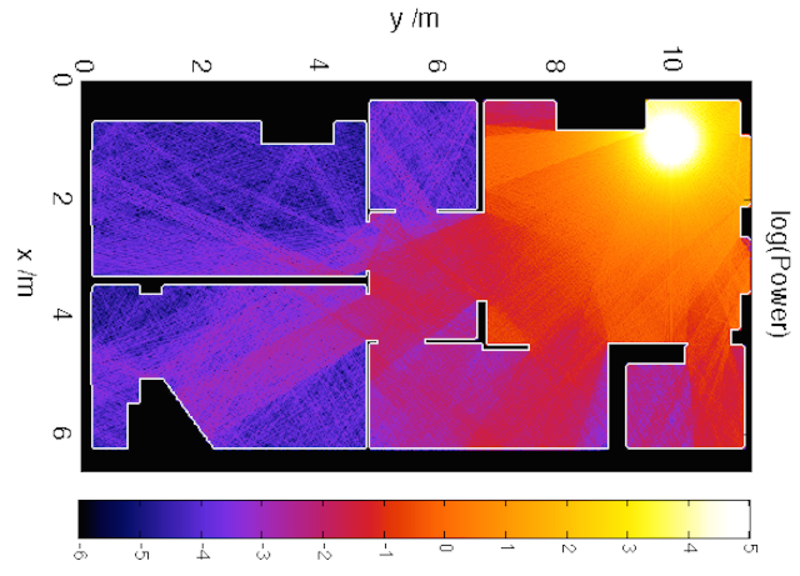
\includegraphics[scale=0.3]{images/wifi-propagation.png}
    \end{center}
  \subsection{Méthodes}
    On peut diviser les méthodes de localisation en deux catégories bien distinctes.

    Nous avons dans un premier temps, les méthodes dites de «~propagation~» qui se basent sur la connaissance préalable de l'ensemble des points d'accès
	\textit{Wifi} qui seront utilisés ainsi que sur la qualité du signal que reçoit l'utilisateur pour pouvoir déterminer la position exacte de ce dernier.

    Les méthodes de la deuxième catégorie parviennent, quand à elle, à localiser l'utilisateur en calculant la similarité entre une mesure (ensemble de
	\textit{Wifi}) donnée et une mesure présente en base de données et qui a été faite ultérieurement.\\  % ultérieurement ? Pas précédemment ?
    Ces méthodes seront discutées et expliquées dans les deux sous-sections suivante.

    \subsubsection{Trilatération}
      La trilatération est une méthode mathématique permettant de trouver une coordonnée \textit{consensus} qui sera contenu dans l'intersection de trois
	  cercles. À la différence de la triangulation, la trilatération est basée sur l'utilisation de trois distances alors que la triangulation utilise
	  trois angles donnés. Le schéma typique d'une trilatération est représenté par la figure~\ref{fig:trilatération}.

	  \begin{figure}
	  	\label{fig:trilatération}
        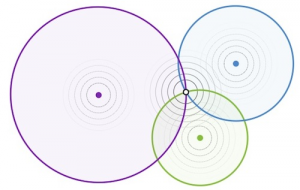
\includegraphics[scale=0.8]{images/trilateration.png}
      \end{figure}

	  Plus formellement, pour déterminer la position d'un utilisateur sur un plan cartésien, nous devons disposer des coordonnées cartésiennes du centre
	  de chaque cercle ainsi que de la distance entre l'utilisateur et ces centres comme mentionné plus haut. L'obtention des coordonnées cartésiennes
	  de l'utilisateur est réalisée via les formules suivante (voir annexe+NUMÉRO pour le développement détaillé)~:
      \begin{equation}
        x = \frac{CE-BF}{EA-BD}
      \end{equation}
      \begin{equation}
        y = \frac{FA-DC}{EA-BD},
      \end{equation}
      où :
      \begin{itemize}
        \item $A = 2x_{2}-2x_{1}$
        \item $B = 2y_{2}-2y_{1}$
        \item $C = r_{1}^{2}-r_{2}^{2}-y_{1}^{2}+y_{2}^{2}-x_{1}^{2}+x_{2}^{2}$
        \item $D = 2x_{3}-2x_{2}$
        \item $E = 2y_{3}-2y_{2}$
        \item $F = r_{2}^{2}-r_{3}^{2}-y_{2}^{2}+y_{3}^{2}-x_{2}^{2}+x_{3}^{2}$
      \end{itemize}

      L'adaptation de la trilatération au problème de localisation se fait en déterminant la distance séparant l'utilisateur d'un point d'accès \textit{Wifi}
	  (centre de cercles). On obtient la distance entre un récepteur (utilisateur) et un émetteur via une fonction qui prend en paramètre la qualité de signal
	  de l'émetteur perçu par le récepteur. La fonction est la suivante~:
      \begin{equation}\label{eq:distance function from signal}
        \alpha_f(s) = \frac{27,55-20\log_{10}(f)+\abs s}{20}
      \end{equation}
      \begin{equation}
        d_f(s) = 10^{\alpha_f(s)},
      \end{equation}
      où :
      \begin{itemize}
        \item $f$ est la fréquence (généralement 2.4 Ghz ou 5.0 GHz)~;
        \item $s$ est la qualité du signal (mesuré en $\dBm$).
      \end{itemize}

      \begin{figure}
        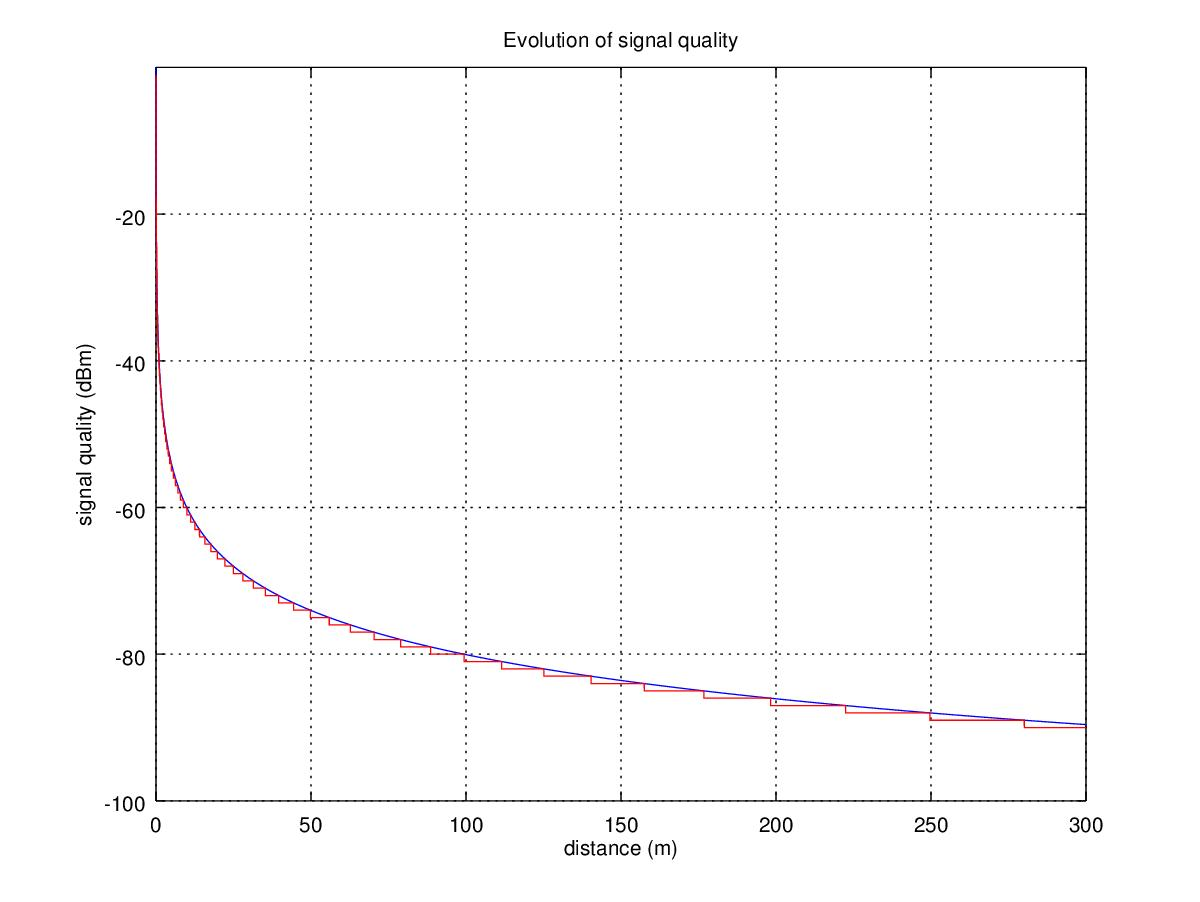
\includegraphics[scale=0.4]{images/signal-propagation.jpg}
        \caption{Répartition de la qualité de signal en fonction de la distance.}
      \end{figure}

	  L'utilisation d'une telle fonction donne de bons résultats dans un environnement ouvert ou les obstacles sont rares. Comme démontré par \cite{Roumanie},
	  la précision de la localisation est situé entre $2$ et $2.5$ mètres. Néanmoins, dans le cas contraire, la fonction d'évaluation de la distance ne prenant
	  pas en compte les obstacles, les estimations de distance s'en retrouvent biaisées et les coordonnées supposées de l'utilisateur aussi. De manière à résoudre
	  ce problème, il est possible de remplacer la constante dans la formule~\eqref{eq:distance function from signal} par une formule prenant en compte les éléments
	  composant l'environnement. Cette formule est définie comme suit~:
      \begin{equation}
        \text{PLACER QQCH ICI}
      \end{equation}

	  Cette modification de la trilatération implique de disposer de plus de connaissance sur l'environnement. Collecter ces données demande du temps et même en
	  consentant à les collecter, les estimations de distance laissent à désirer.

    \subsubsection{Localisation via une \textit{Signal Strength Map}}
      Une \textit{SSM} est défini comme étant une cartographie des régions couvertes par les signaux \textit{Wifi}. La construction de cette carte se fait en regardant
	  et enregistrant quels sont les points d'accès \textit{Wifi} que l'on capte à une certaine position. On va donc enregistrer, dans une base de données, pour chaque
	  position désirée, les identifiants (\textit{BSS}) et les qualités de signal des points d'accès \textit{Wifi} couvrant cette position.

	  \paragraph{Méthode utilisant les processus Gaussiens}

	  \paragraph{Méthode utilisant les maximum de vraisemblance}
        Comme mentionné plus haut, on va faire un ensemble de mesures pour chaque point du graphe et ainsi construire la base de données sur laquelle se basera notre
		méthode de localisation. Pour la méthode présente, on notera une mesure comme suit~:
        \begin{equation}
          S^{(i)}=\{b_{1}, b_{2}, ..., b_{n}\} \hspace{1cm} \forall j \in [1, k],  % soucis d'indices... Qu'est-ce que $j$ ?
        \end{equation}
        où :
        \begin{itemize}
          \item $n$ est le nombre de points d'accès détectés lors de la mesure~;
          \item $b_{i}$, le $i^{eme}$ point d'accès détecté, est défini comme un couple $(a_{i}, S_{i})$ décrivant respectivement l'identifiant d'un point d'accès
		  et la qualité de signal perçue.
        \end{itemize}

        On prend plusieurs mesures pour un même point car il existe des variations de qualité de signal au cours du temps. En faisant de la sorte, on se donne une idée de
		la qualité d'un signal à un point du graphe. On notera ces «~mesures moyennes~» comme suit~:
        \begin{equation}
          \bar{S} = \{(a_{1}, \bar{S}_{1}), ..., (a_{n}, \bar{S}_{n})\},
        \end{equation}
        où :
        \begin{itemize}
          \item $\bar{S}_{i} = \frac{1}{k}\sum\limits_{j = 1}^{k} S_{i}^{i} \hspace{1cm} \forall i \in [1, n]$
        \end{itemize}

		Cependant, considérer seulement la moyenne comme utile statistique n'est pas suffisant à cause du bruit et des interférences pouvant survenir (voir section précédente).
		Pour palier ce problème, on calcule aussi la variance (notée $v$) pour chaque point du graphe. Ainsi, on obtiendra une nouvelle forme appelée ensemble caractéristique
		qui est définit comme suit :
        \begin{equation}
          S^{*} = \{(a_{1}, \bar{S}_{1}, v_{1}), ..., (a_{n}, \bar{S}_{n}, v_{n})\}
        \end{equation}
        Où :
        \begin{itemize}
          \item $v_{i} = \frac{1}{k-1}\sum\limits_{j = 1}^{k}(S_{i}^{(j)}-\bar{S}_{i}) \hspace{1cm} \forall i \in [1,n]$.
        \end{itemize}
        On peut donc définir notre base de données (notée $\mathcal{D}$) comme l'ensemble des points du graphe (noté $L$) pour lesquels il existe un ensemble caractéristique.
		Soit~:
        \begin{equation}
          \mathcal{D} = \{L_{1}, L_{2}, ..., L_{3}\},
        \end{equation}
        où :
        \begin{itemize}
          \item $\dim(L_{i})$, le nombre de points d'accès à cette position, est noté $n_{i}$
          \item $S_{i}^{*}$ est l'ensemble caractéristique de $L_{i}$
        \end{itemize}

        Une fois la base de données remplie, on peut passer à l'étape dite d'exploitation. Il s'agit du processus qui sera utilisé par une personne pour pouvoir se localiser.
        Le processus va déduire la position de l'utilisateur sur base de la base de données préalablement créée (notée $\mathcal{D}$) et sur base d'une mesure qu'il aura effectuée
		(notée $S'$). La nature de cette mesure pouvant soit être de la forme (1) ou (2).

        Le processus va déterminer une position $\hat{L}$ appartenant $\mathcal{D}$ pour laquelle la probabilité que l'utilisateur se trouve proche de ce point est la plus grande.
		Pour ce faire, on va calculer, pour chaque élément appartenant à $\mathcal{D}$, un score noté $Z$ et considérer, comme solution à notre problème, le point correspondant
		au score $Z$ minimal car le score $Z$ minimal représente la vraisemblance maximale comme prouvé dans l'article (Mettre référence). Le score $Z$ est définit comme suit~:
        \begin{equation}
          Z_{i} = \sum\limits_{j = 1}^{n_{i}}\bigg(\frac{(\bar{S}_{ij}-S'_{j})^{2}}{v_{ij}}\bigg),
        \end{equation}
        où :
        \begin{itemize}
          \item $\bar{S}_{ij}$ est la moyenne de la qualité de signal du $j^{eme}$ point d'accès~;
          \item $v_{ij}$ est la variance de la qualité de signal du $j^{eme}$ point d'accès~;
          \item $S'_{j}$ est la qualité de signal du $j^{eme}$ point d'accès de la mesure effectué par l'utilisateur.
        \end{itemize}

        \begin{tcolorbox}[title = Mesures parasites]
          Dans cet article, on défini une mesure parasite comme la détection d'un point d'accès qui n'apparaitrait que très rarement lors de la prise de mesures. On qualifiera
		  un point d'accès comme tel si le nombre de fois qu'il a été détecté est inférieur à un seuil fixé.
          Ce cas de figure survient pour des points d'accès situés à une distance telle qu'ils ne sont pas toujours perçus mais qui, dans le cas contraire, présentent des qualités
		  de signal inférieur à $-90 dBm$.
        \end{tcolorbox}

      \paragraph{Monte Carlo}
      \paragraph{Amélioration par l'utilisation de filtres}
      \paragraph{Amélioration par l'estimation de qualité de signal}

\section{Interpolation}
  \subsection{Principe}
  \subsection{Interpolation polynômiale}
  \subsection{Interpolation par morceaux}  % piece-wise interpolation
\section{Discussion et limitations}
\section{Conclusion}

\begin{thebibliography}{9}
  \bibitem{ssm}
    Matteo Cypriani, Frédéric Lassabe, Philippe Canalda, François Spies,
    \emph{Wi-Fi-Based Indoor Positioning: Basic Techniques, Hybrid Algorithms and Open Software Platform}.
    2010.
  \bibitem{Roumanie}
    Bianca BOBESCU, Marian ALEXANDRU
    \emph{Mobile indoor positioning using Wi-fi localisation}.
    Transilvania University, Brasov, Romania,
    2015.
  \bibitem{trilateration}
    OnkarPathak, Pratik Palaskar, Rajesh Palkar, Mayur Tawari,
    \emph{Wi-Fi Indoor Positioning System based on RSSI Measurements from Wi-Fi Access Points A Trilateration Approach}.
    International Journal of Scientific \& Engineering Research,
    2014.
  \bibitem{GaussianProcessesFerris}
    Brian Ferris, Dirk Hähnel, Dieter Fox,
    \emph{Gaussian Processes for Signal Strength-Based Location Estimation}.
    University of Washington, Department of Computer Science \& Engineering, Seattle, WA Intel Research Seattle, Seattle, WA.
  \bibitem{ETH}
    Thomas Locher, Roger Wattenhofer, Aaron Zollinger,
    \emph{Received-Signal-Strength-Based Logical Positioning Resilient to Signal Fluctuation}.
    Computer Engineering and networks Laboratory, ETH zurich, Switzerland.
\end{thebibliography}

%---------- SCANNING ----------
%# www.mdpi.com/1424-8220/15/9/21824/pdf
%https://www.researchgate.net/publication/224198838_Wi-Fi-based_indoor_positioning_Basic_techniques_hybrid_algorithms_and_open_software_platform
%x https://fruct.org/publications/abstract16/files/Shc1.pdf
%http://www.afahc.ro/ro/revista/2015_1/119.pdf
%x http://file.scirp.org/pdf/CN_2013071010352139.pdf
%http://www.ijser.org/researchpaper%5CWi-Fi-Indoor-Positioning-System-Based-on-RSSI-Measurements.pdf
%https://www.researchgate.net/profile/Suhailan_Safei/publication/230771403_INDOOR_POSITION_DETECTION_USING_WIFI_AND_TRILATERATION_TECHNIQUE/links/5513e9120cf2eda0df3031f0.pdf
%http://www.ee.ucl.ac.uk/lcs/previous/LCS2005/12.pdf
%http://www.int-arch-photogramm-remote-sens-spatial-inf-sci.net/XXXVIII-4-C26/1/2012/isprsarchives-XXXVIII-4-C26-1-2012.pdf
%---------- LOCALISATION ----------
%http://www.roboticsproceedings.org/rss02/p39.pdf
%https://venturi.fbk.eu/wp-content/uploads/2011/10/AraMes_WIMOB_2014.pdf
%http://www.tik.ee.ethz.ch/file/2490a7adb6a163b9c5be1510d033870a/sawn05.pdf
%https://felixduvallet.github.io/pubs/2008-WiFi-IROS.pdf
%http://www.cs.cmu.edu/~mmv/papers/10icra-joydeep.pdf
%https://papers.nips.cc/paper/2541-gpps-a-gaussian-process-positioning-system-for-cellular-networks.pdf
%http://www-cs.stanford.edu/people/dstavens/icra11/huang_etal_icra11.pdf
%https://www.ncbi.nlm.nih.gov/pmc/articles/PMC5017359/
%http://www.robot.t.u-tokyo.ac.jp/~yamashita/paper/E/E293Final.pdf

\section*{Annexes}
  \subsection*{A. Algorithme de Dijkstra}
    L'idée de l'algorithme de Dijkstra est de conserver un vecteur des nœuds à traiter contenant initialement tous les nœuds, et duquel on enlève chaque nœud
    lorsqu'il est traité. Afin de choisir le nœud à traiter à chaque étape, il faut regarder lequel de ces nœuds nécessite un coût minimal pour être atteint
    depuis la source. C'est ainsi que l'algorithme de Dijkstra assure de déterminer un chemin optimal dans le graphe. L'algorithme peut être schématisé comme suit~:

\begin{verbatim}
set all distances to infty
set src distance to 0
Q <- priority queue
Q.addAll(nodes)
WHILE NOT Q.empty()
  N <- Q.pop()
  IF N == dest
    RETURN the path from src to dest
  ELSE
    FOR EACH N' IN N.neighbours()
      update distance to N'
      update closest node leading to N'
    END FOR EACH
  END IF
END WHILE
\end{verbatim}

\end{document}
